% The House Always Wins: Gambling in America
% Compile with: latexmk -pdf gambling.tex
\documentclass[aspectratio=169,11pt]{beamer}

\usepackage[T1]{fontenc}
\usepackage{lmodern}
\usepackage{textcomp}
\usepackage{booktabs}
\usepackage{array}
\usepackage{tikz}
\usetikzlibrary{shapes.geometric,positioning,calc,arrows.meta}
\usepackage{pgfplots}
\pgfplotsset{compat=1.18}
\usepackage[most]{tcolorbox}
\graphicspath{{images/}}

% ---------- Colors ----------
\definecolor{navy}{HTML}{1C2541}
\definecolor{oldred}{HTML}{B22234}   % US flag red, also the accent color
\definecolor{oldblue}{HTML}{3C3B6E}  % US flag blue
\definecolor{ink}{HTML}{2B2B2B}
\definecolor{muted}{HTML}{8A8F98}
\definecolor{paper}{HTML}{FFFFFF}
\definecolor{dem}{HTML}{2E5FA3}      % Democrats
\definecolor{rep}{HTML}{C0392B}      % Republicans
\definecolor{austria}{HTML}{C8102E}  % Austria red, for USA-vs-Austria comparisons

% ---------- Minimal theme ----------
\setbeamertemplate{navigation symbols}{}
\setbeamercolor{normal text}{fg=ink, bg=paper}
\setbeamercolor{structure}{fg=navy}
\setbeamercolor{frametitle}{fg=navy}
\setbeamercolor{alerted text}{fg=oldred}
\setbeamercolor{footnote}{fg=muted}
\setbeamerfont{frametitle}{size=\Large, series=\bfseries}
\setbeamertemplate{itemize item}{\color{oldred}\textbullet}
\setbeamertemplate{itemize subitem}{\color{muted}--}
\setbeamertemplate{enumerate item}{\color{oldred}\insertenumlabel.}
\setbeamersize{text margin left=1.1cm, text margin right=1.1cm}
\hypersetup{colorlinks=true, urlcolor=dem, linkcolor=navy}

\setbeamertemplate{frametitle}{%
  \vspace*{0.5cm}%
  \usebeamerfont{frametitle}\usebeamercolor[fg]{frametitle}\insertframetitle\par
  \vspace{0.15cm}{\color{navy!15}\rule{\textwidth}{0.4pt}}\par}

\setbeamertemplate{footline}{%
  \hfill{\tiny\color{muted}\insertframenumber}\hspace*{0.6cm}\vspace*{0.35cm}}

% Plain divider at the start of each section
\AtBeginSection{%
  \begin{frame}[plain,noframenumbering]
    \centering
    {\LARGE\bfseries\color{navy}\insertsection}\\[0.6em]
    {\color{oldred}\rule{1.5cm}{0.8pt}}
  \end{frame}}

% "Think" question slides: \begin{thinkframe} ... \end{thinkframe}
\newenvironment{thinkframe}{%
  \begin{frame}[plain,noframenumbering,environment=thinkframe]\centering\Large}{\end{frame}}

% ---------- Helpers ----------
% Small grey source line at the bottom of a frame
\newcommand{\source}[1]{%
  \begin{tikzpicture}[remember picture,overlay]
    \node[anchor=south west, font=\tiny, text=muted, text width=0.85\paperwidth, align=left]
      at ($(current page.south west)+(0.6cm,0.25cm)$) {#1};
  \end{tikzpicture}}

% Quote box with a thin red rule on the left; optional arg e.g. [fontupper=\itshape\small]
\newtcolorbox{textquote}[1][]{%
  enhanced, frame hidden, boxrule=0pt, sharp corners,
  colback=navy!4, borderline west={2pt}{0pt}{oldred},
  left=10pt, right=8pt, top=6pt, bottom=6pt, fontupper=\itshape, #1}

% Photo + name + short bio (use inside a column): \candidate{file}{Name}{bio}
\newcommand{\candidate}[3]{%
  \begin{minipage}[t]{\linewidth}\centering
    \includegraphics[height=3.5cm]{#1}\\[0.5em]
    {\large\bfseries\color{navy}#2}\\[0.4em]
    \begin{minipage}{0.9\linewidth}\raggedright\small #3\end{minipage}
  \end{minipage}}

% Big number with a caption (use inside a column): \bignum{color}{91\%}{caption}
\newcommand{\bignum}[3]{%
  \begin{minipage}[t]{\linewidth}\centering
    {\fontsize{34}{38}\selectfont\bfseries\color{#1}#2}\\[0.3em]
    {\small #3}
  \end{minipage}}

% US flag drawn in TikZ (hoist height = #1), e.g. \usflag{3cm}
\newcommand{\usflag}[1]{%
  \begin{tikzpicture}[x=#1, y=#1]
    \def\fly{1.9}
    \foreach \i in {0,...,12} {
      \pgfmathsetmacro{\c}{mod(\i,2)==0 ? 1 : 0}
      \ifdim\c pt=1pt
        \fill[oldred] (0,{1-(\i+1)/13}) rectangle (\fly,{1-\i/13});
      \else
        \fill[white] (0,{1-(\i+1)/13}) rectangle (\fly,{1-\i/13});
      \fi
    }
    \def\cw{0.76} \def\ch{0.5385}
    \fill[oldblue] (0,{1-\ch}) rectangle (\cw,1);
    \foreach \r in {1,...,9} {
      \pgfmathsetmacro{\isodd}{mod(\r,2)}
      \ifdim\isodd pt=1pt
        \foreach \k in {0,...,5}
          \node[star, star points=5, star point ratio=2.618, fill=white, inner sep=0pt,
                minimum size=0.0616*#1] at ({(2*\k+1)*\cw/12},{1-\r*\ch/10}) {};
      \else
        \foreach \k in {0,...,4}
          \node[star, star points=5, star point ratio=2.618, fill=white, inner sep=0pt,
                minimum size=0.0616*#1] at ({(2*\k+2)*\cw/12},{1-\r*\ch/10}) {};
      \fi
    }
    \draw[ink!30, line width=0.3pt] (0,0) rectangle (\fly,1);
  \end{tikzpicture}}

% Agree/disagree spectrum for "spectrum game" activities
\newcommand{\spectrum}{%
  
\begin{tikzpicture}
    \shade[left color=oldblue, right color=oldred, rounded corners=2pt] (0,0) rectangle (11,0.18);
    \node[anchor=north, font=\small, text=oldblue] at (0,-0.15) {Strongly disagree};
    \node[anchor=north, font=\small, text=muted] at (5.5,-0.15) {Neutral};
    \node[anchor=north, font=\small, text=oldred] at (11,-0.15) {Strongly agree};
    \fill[paper, draw=muted] (5.5,0.09) circle (2.5pt);
  \end{tikzpicture}}

% One statement per slide: \statement{number}{total}{text}
\newcommand{\statement}[3]{%
  \begin{frame}[plain]
    \vfill
    \begin{center}
      {\small\color{muted}Statement #1 of #2}\\[1.2em]
      {\LARGE\bfseries #3}
    \end{center}
    \vfill
    \begin{center}\spectrum\end{center}
    \vspace{1.2cm}
  \end{frame}}


% ---------- Helpers for this deck ----------
\newcommand{\ans}[1]{{\color{oldred}\bfseries #1}}
% Two-column slide body: \textpic{bullets}{image}{caption}
\newcommand{\textpic}[3]{%
  \begin{columns}[c,onlytextwidth]
    \begin{column}{0.52\textwidth}\raggedright #1\end{column}
    \begin{column}{0.44\textwidth}\centering
      \includegraphics[width=\linewidth,height=4.9cm,keepaspectratio]{#2}\\[0.2em]
      {\tiny\color{muted} #3\par}
    \end{column}
  \end{columns}}
% One slide per sentence, answer on click: \casino{n}{sentence}{answer}
\newcommand{\casino}[3]{%
  \begin{frame}[plain]
    \vfill
    \begin{center}
      {\small\color{muted}Grammar Casino: #1 of 14}\\[1.4em]
      {\LARGE\bfseries\color{navy} #2\par}
      \vspace{1.6em}
      \onslide<2->{{\Large #3\par}}
    \end{center}
    \vfill
  \end{frame}}
\newcommand{\cright}{\ans{Correct!}}

\begin{document}

\begin{frame}[plain]
  \begin{columns}[c,onlytextwidth]
    \begin{column}{0.52\textwidth}
      {\fontsize{30}{34}\selectfont\bfseries\color{navy} The House\\Always Wins\par}\vspace{0.6em}
      {\Large\color{muted} Gambling in America}\\[0.6em]
      {\color{oldred}\rule{3cm}{1.5pt}}
    \end{column}
    \begin{column}{0.44\textwidth}
      \centering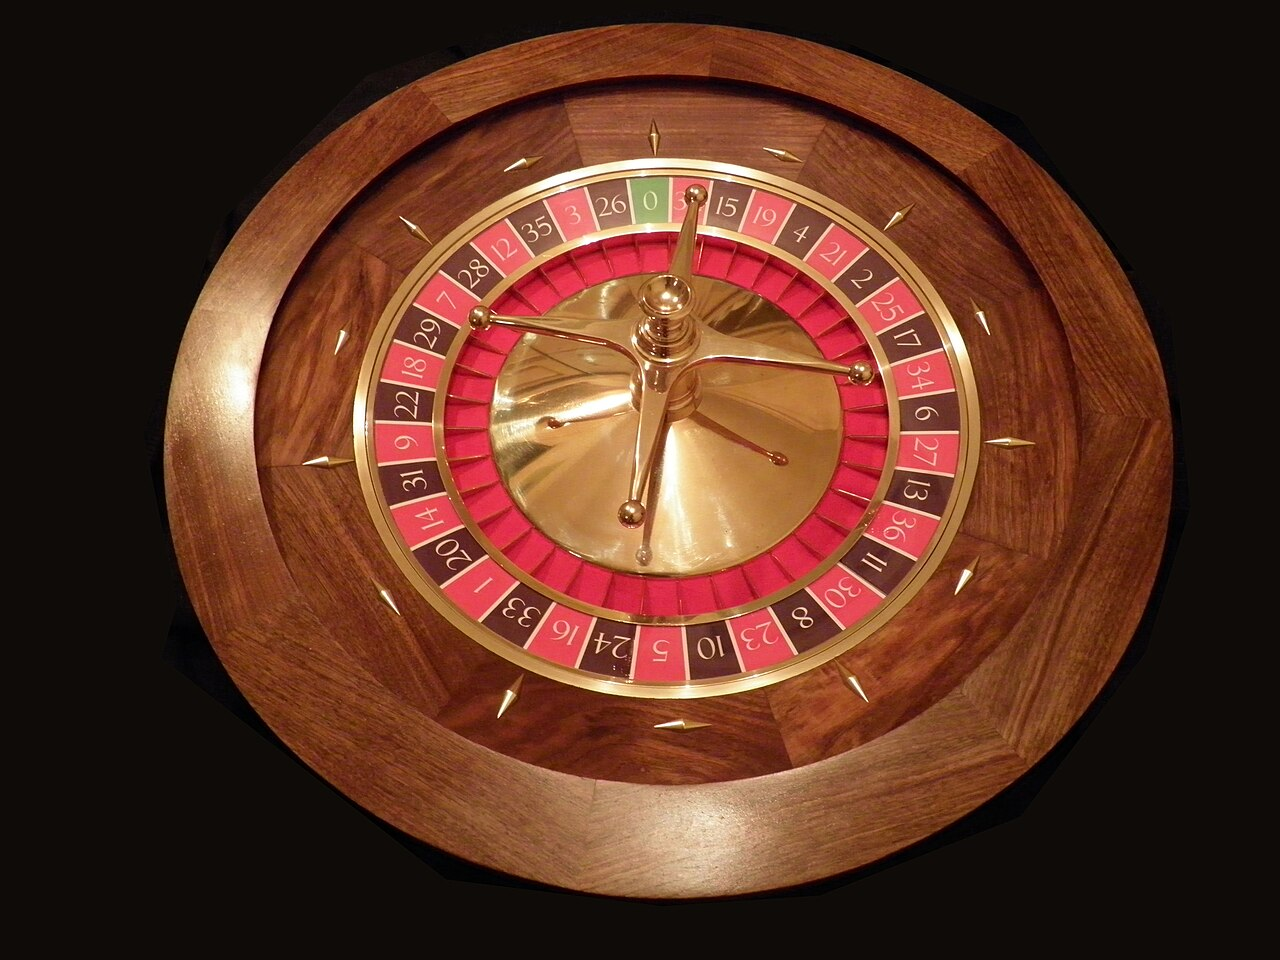
\includegraphics[width=\linewidth]{roulette.jpg}\\[0.2em]
      {\tiny\color{muted} Photo: Oniff, CC BY-SA 4.0\par}
    \end{column}
  \end{columns}
\end{frame}

% =====================================================================
\section{Is It Legal?}

\begin{frame}{Stand up if you think so}
  \centering
  {\LARGE\bfseries Is gambling legal in the USA?}\\[1.4em]
  {\Large Stand = \alert{yes} \qquad Sit = \alert{no}}
\end{frame}

\begin{frame}[plain]
  \begin{columns}[c,onlytextwidth]
    \begin{column}{0.5\textwidth}
      {\fontsize{30}{34}\selectfont\bfseries\color{navy} It's\\complicated.\par}
    \end{column}
    \begin{column}{0.45\textwidth}
      \centering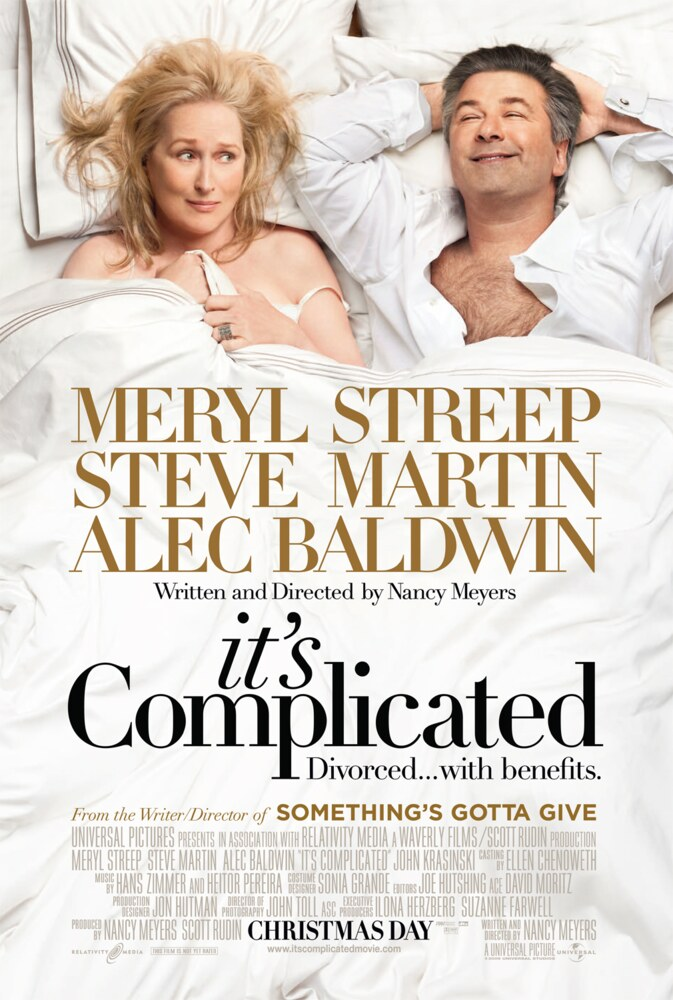
\includegraphics[height=0.86\paperheight]{complicated.jpg}
    \end{column}
  \end{columns}
\end{frame}

\begin{frame}[plain]
  \begin{tikzpicture}[remember picture,overlay]
    \node at (current page.center) {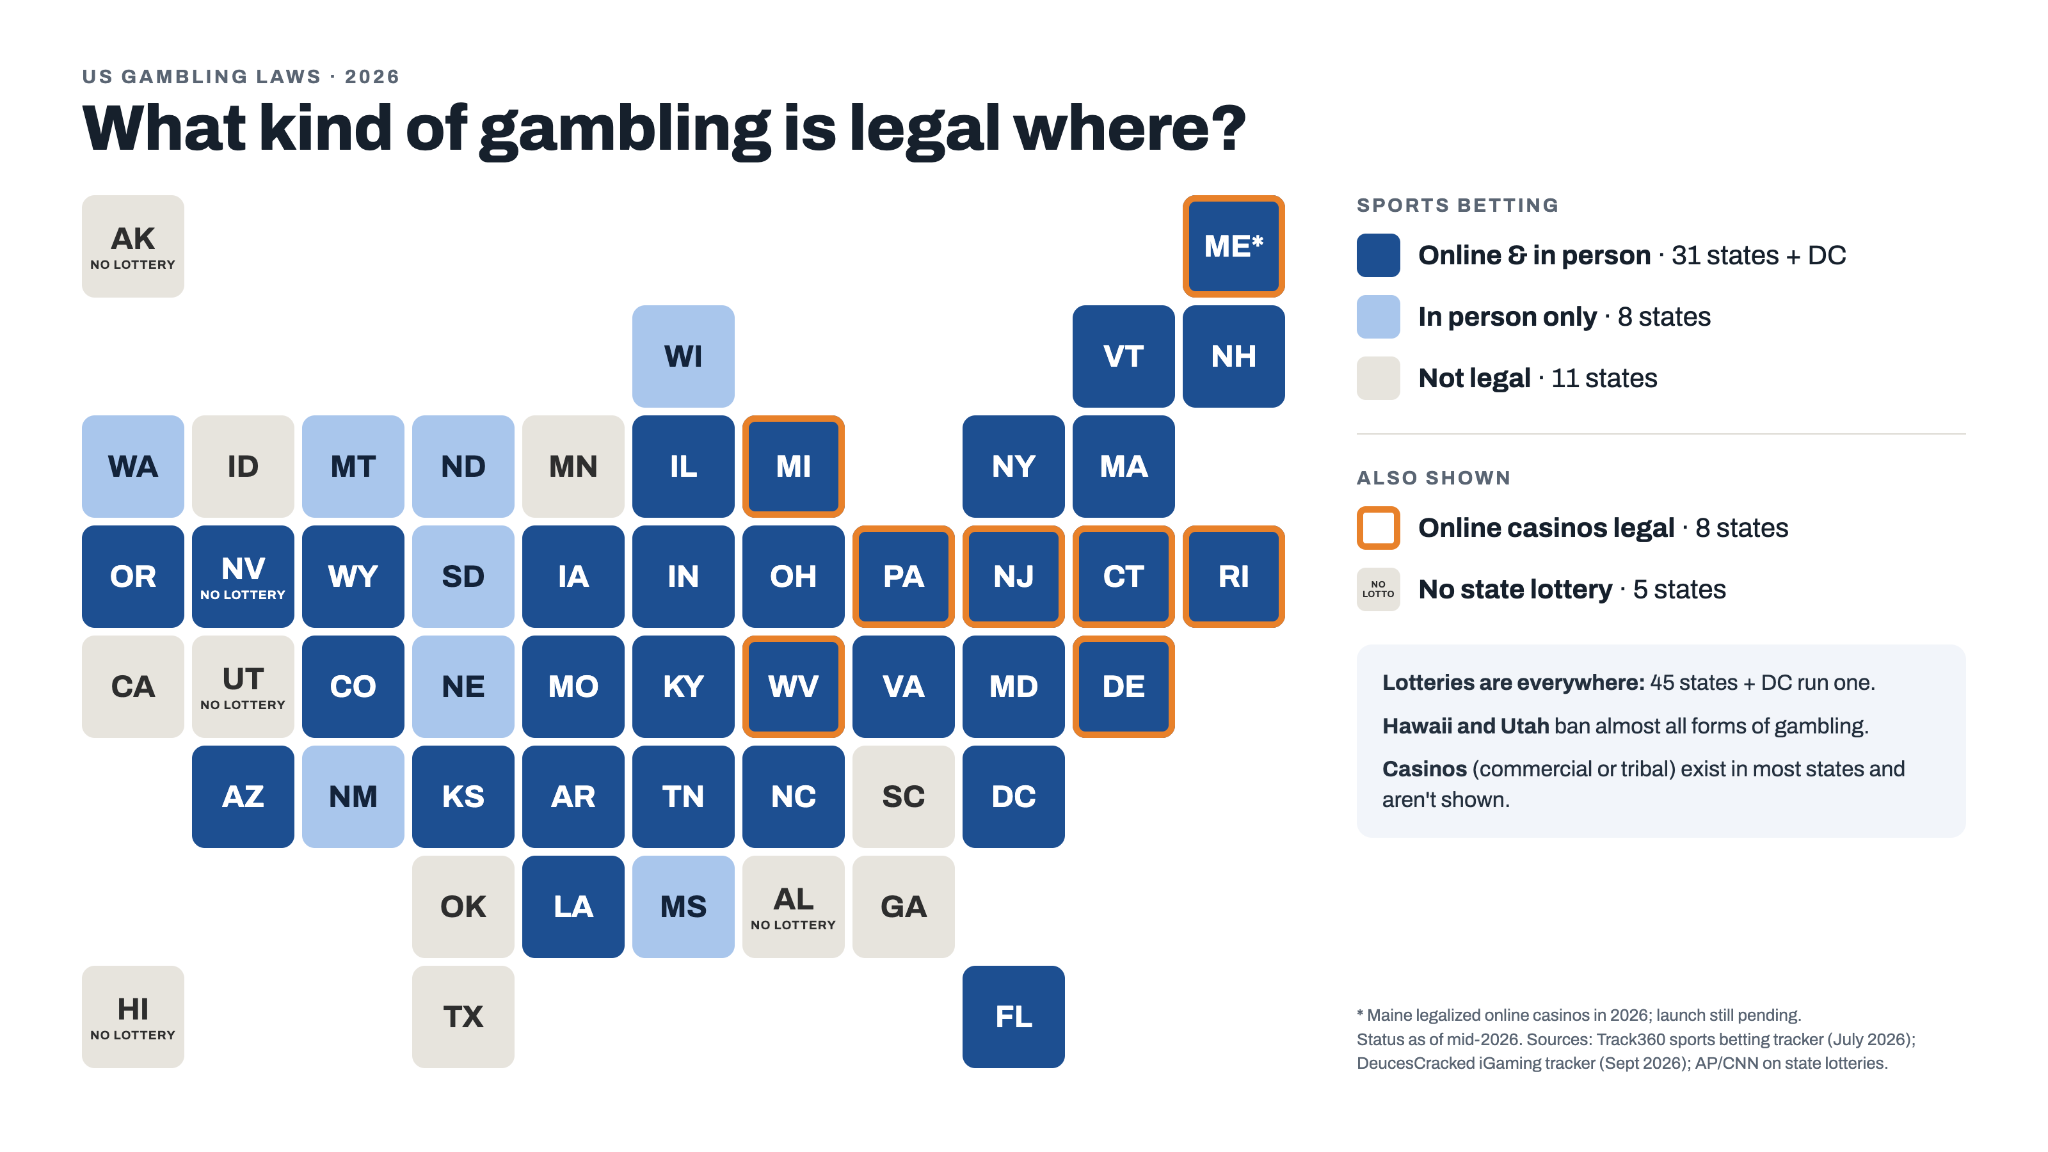
\includegraphics[width=\paperwidth]{map.png}};
  \end{tikzpicture}
\end{frame}

\begin{frame}{Native American casinos}
  \textpic{\begin{itemize}\setlength{\itemsep}{0.7em}
    \item Tribes are \alert{sovereign nations}
    \item They can run casinos
    \item 246 tribes, in 29 states
    \item 2025 revenue: \alert{\$46.2 billion}
    \item Money for schools, health, housing
  \end{itemize}}{foxwoods.jpg}{Foxwoods, run by the Mashantucket Pequot (Connecticut).\\Photo: Stilfehler, CC BY-SA 3.0}
  \source{Source: National Indian Gaming Commission (FY 2025).}
\end{frame}

\begin{frame}{The grey market}
  \textpic{\begin{itemize}\setlength{\itemsep}{0.7em}
    \item Bet on almost \alert{anything}
    \item Elections, wars, MrBeast views
    \item Companies: ``It's not gambling''
    \item States: ``Yes, it is''
    \item Courts \alert{disagree} with each other
  \end{itemize}}{polymarket.jpg}{Screenshot: Polymarket, October 2026}
  \source{Source: Al Jazeera (Sept. 2026); Front Office Sports (2026).}
\end{frame}

\begin{frame}{Vote: should this be legal?}
  \relax{\large\color{muted} Hands up for yes\par}
  \vspace{0.8em}
  \begin{itemize}\setlength{\itemsep}{0.9em}\large
    \item<1-> Betting on a football match
    \item<2-> Betting on an election
    \item<3-> Betting on a \alert{war}
    \item<4-> Betting on your teacher's lateness
  \end{itemize}
\end{frame}

% =====================================================================
\section{The Games}

\begin{frame}{Which is most popular?}
  \centering
  {\LARGE\bfseries\color{navy} Lottery \quad Casino \quad Sports betting}\\[1.4em]
  {\fontsize{30}{34}\selectfont\bfseries\color{oldred} 31\% \quad 15\% \quad 14\%}\\[1.2em]
  {\large\color{muted} Percent of US adults, past year. Match them!}
\end{frame}

\begin{frame}{Which is most popular?}
  \centering
  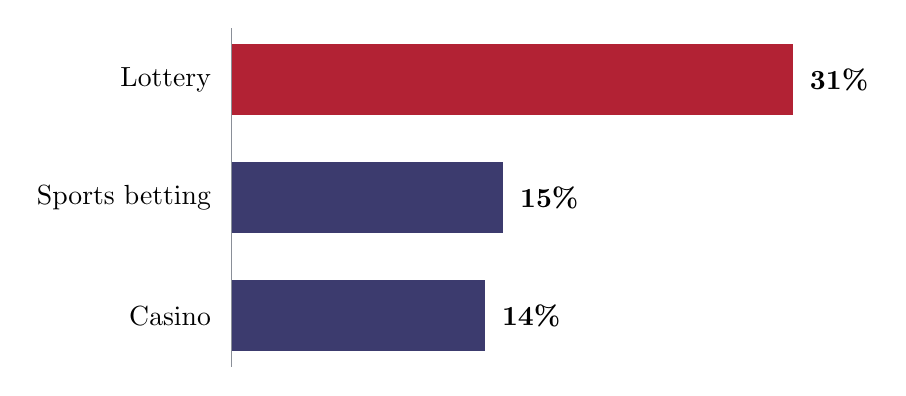
\begin{tikzpicture}[x=0.23cm]
    \foreach \y/\lab/\val/\col in {3/Lottery/31/oldred, 1.5/Sports betting/15/oldblue, 0/Casino/14/oldblue} {
      \fill[\col] (0,\y) rectangle (\val,\y+0.9);
      \node[anchor=east] at (-0.6,\y+0.45) {\lab};
      \node[anchor=west, font=\bfseries] at (\val+0.4,\y+0.45) {\val\%};
    }
    \draw[muted] (0,-0.2) -- (0,4.1);
  \end{tikzpicture}
  \source{Source: Gallup, telephone survey of US adults, June--July 2026.}
\end{frame}

\begin{thinkframe}
  {\color{oldred}\textbf{The house edge}}\\[0.8em]
  For every \texteuro 100 you bet, how much does the casino keep,\\
  on average, in the long run?
\end{thinkframe}

\begin{frame}{Rank them: best to worst for you}
  \begin{itemize}\setlength{\itemsep}{0.9em}\large
    \item Roulette (European wheel)
    \item Blackjack (perfect play)
    \item Slot machines
    \item Baccarat: bet on a tie
    \item All US sports bets
  \end{itemize}
\end{frame}

\begin{frame}{What the house keeps from every 100}
  \centering
  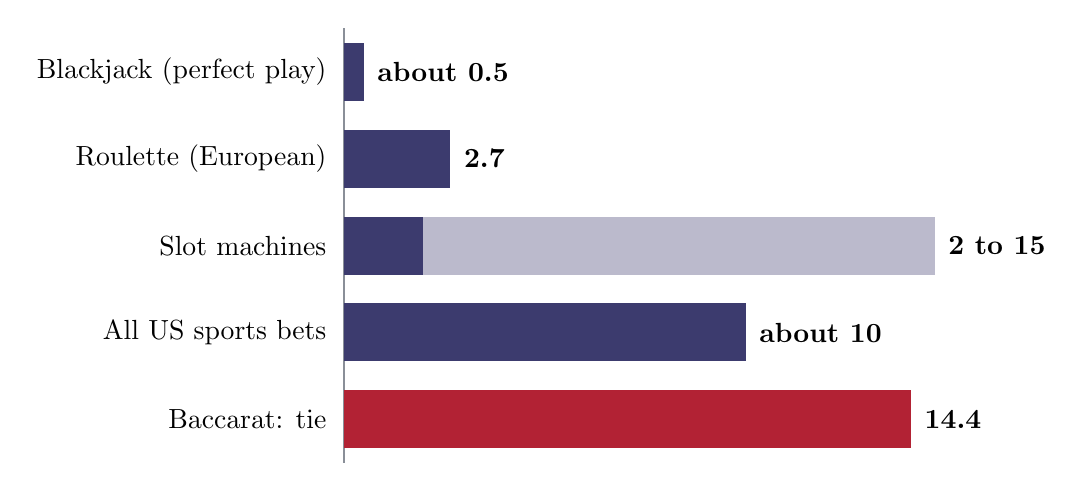
\begin{tikzpicture}[x=0.5cm,y=0.92cm]
    \foreach \y/\lab in {4.8/{Blackjack (perfect play)}, 3.6/Roulette (European), 2.4/Slot machines, 1.2/All US sports bets, 0/Baccarat: tie}
      \node[anchor=east] at (-0.2,\y+0.4) {\lab};
    \draw[muted] (0,-0.2) -- (0,5.8);
    \onslide<2->{
    \foreach \y/\val/\lab/\col in {4.8/0.5/about 0.5/oldblue, 3.6/2.7/2.7/oldblue, 1.2/10.2/about 10/oldblue, 0/14.4/14.4/oldred} {
      \fill[\col] (0,\y) rectangle (\val,\y+0.8);
      \node[anchor=west, font=\bfseries] at (\val+0.1,\y+0.4) {\lab};
    }
    \fill[oldblue] (0,2.4) rectangle (2,3.2);
    \fill[oldblue!35] (2,2.4) rectangle (15,3.2);
    \node[anchor=west, font=\bfseries] at (15.1,2.8) {2 to 15};
    }
  \end{tikzpicture}
  \source{Sports: share actually kept, 2025 (\$17.0bn of \$166.9bn bet; American Gaming Association). US roulette: 5.3.}
\end{frame}

\begin{frame}{Lottery: how likely is the jackpot?}
  \textpic{{\Large 1 in \ldots ?\par}\vspace{0.8em}
    {\large A) 290,000\\[0.5em] B) 29 million\\[0.5em] C) \only<1>{290 million}\only<2->{\ans{290 million}}\par}
    \vspace{1em}One ticket: \$5\\[0.6em]
    \href{https://www.youtube.com/watch?v=8LSj-W7WUpA}{Watch a drawing}
  }{megamillions.jpg}{Old Mega Millions tickets (2012). Photo: Lieutenant Ramathorn, CC0}
  \source{Source: Mega Millions, via Yahoo News.}
\end{frame}

\begin{frame}{Sports betting}
  \textpic{\begin{itemize}\setlength{\itemsep}{0.8em}
    \item Banned almost everywhere until \alert{2018}
    \item Now: a casino in your pocket
    \item Men 18--49 with an account: \only<1>{\textbf{?}}\only<2->{\ans{52\%}}
  \end{itemize}}{sportsbook.jpg}{Before phones: a Las Vegas sportsbook.\\Photo: Baishampayan Ghose, CC BY-SA 2.0}
  \source{Source: Siena / St.\ Bonaventure survey (April 2026).}
\end{frame}

% =====================================================================
\section{How They Keep You Playing}

\begin{frame}{You run a casino}
  \textpic{{\large Nobody is allowed to leave.\\[0.8em]
    \textbf{How do you keep them playing?}\\[0.8em]
    {\color{muted}Groups, two minutes.\\ No locked doors!}\par}
  }{slots.jpg}{Las Vegas. Photo: Yamaguchi sensei, CC BY-SA 3.0}
\end{frame}

\begin{frame}{Trick 1: Almost!}
  \begin{columns}[c,onlytextwidth]
    \begin{column}{0.5\textwidth}
      \begin{itemize}\setlength{\itemsep}{0.9em}
        \item You lose, but \alert{nearly} win
        \item Your brain reacts like winning
        \item You want to play \alert{more}
      \end{itemize}
    \end{column}
    \begin{column}{0.46\textwidth}
      \centering
      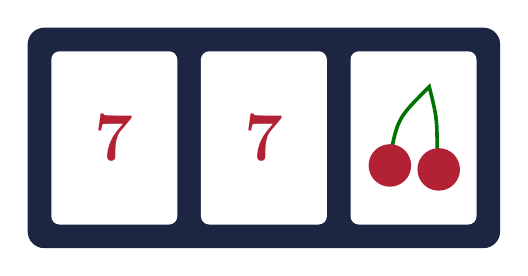
\begin{tikzpicture}
        \fill[navy, rounded corners=6pt] (-0.3,-0.3) rectangle (5.7,2.5);
        \foreach \x in {0,1.9,3.8} \fill[white, rounded corners=3pt] (\x,0) rectangle (\x+1.6,2.2);
        \node[font=\fontsize{38}{40}\selectfont\bfseries, text=oldred] at (0.8,1.1) {7};
        \node[font=\fontsize{38}{40}\selectfont\bfseries, text=oldred] at (2.7,1.1) {7};
        \begin{scope}[shift={(4.6,0.75)}]
          \draw[green!45!black, line width=1.3pt] (-0.3,0.1) .. controls (-0.2,0.6) .. (0.2,1) .. controls (0.3,0.6) .. (0.3,0.1);
          \fill[oldred] (-0.3,0) circle (0.27); \fill[oldred] (0.32,-0.05) circle (0.27);
        \end{scope}
      \end{tikzpicture}
    \end{column}
  \end{columns}
  \source{Source: one brain-scan study, Clark et al., \emph{Neuron} (2009).}
\end{frame}

\begin{frame}{Trick 2: Win or loss?}
  \centering
  {\Large You bet \textbf{75}.\\[0.6em] The machine flashes, sings and pays \textbf{30}.\\[1.1em]
  {\bfseries\color{navy} Did you win?}}\\[1.1em]
  \onslide<2->{{\Large You \ans{lost 45}.}\\[0.4em] {\large Players remember winning more than they did.}}
  \source{Source: Barton et al., \emph{Journal of Gambling Studies} (2017).}
\end{frame}

\begin{frame}{Trick 3: ``Free'' money}
  \begin{columns}[c,onlytextwidth]
    \begin{column}{0.5\textwidth}
      \begin{itemize}\setlength{\itemsep}{0.9em}
        \item It's \alert{credit}, not cash
        \item Cashing out takes more betting
        \item Losing streak? Another bonus
      \end{itemize}
    \end{column}
    \begin{column}{0.44\textwidth}
      \centering
      
\begin{tikzpicture}
        \node[fill=oldred, text=white, rounded corners=8pt, inner sep=14pt, align=center, rotate=4]
          {{\Large Bet \$5}\\[0.3em]{\fontsize{28}{32}\selectfont\bfseries GET \$200!}\\[0.3em]{\tiny Terms and conditions apply. Many, many conditions.}};
      \end{tikzpicture}
    \end{column}
  \end{columns}
  \source{Invented example of a typical offer.}
\end{frame}

\begin{frame}{Trick 4: Your phone calls you}
  \large One customer says DraftKings sent\\[0.5em]
  {\fontsize{30}{36}\selectfont\bfseries\color{oldred}\only<1>{?}\only<2->{about 70}} messages in one month.\\[1em]
  \onslide<2->{\begin{itemize}\setlength{\itemsep}{0.6em}
    \item Emails, texts, notifications
    \item A lawsuit, not yet decided
    \item DraftKings \alert{denies} targeting problem gamblers
  \end{itemize}}
  \source{Source: Boston Globe (Oct.\ 2026). DraftKings says it does not use AI to target customers based on losses or signs of problem gaming.}
\end{frame}

\begin{frame}{Trick 5: Your new best friend}
  \begin{itemize}\setlength{\itemsep}{0.9em}\large
    \item Lose a lot $\rightarrow$ become a \alert{VIP}
    \item A personal ``host'' texts you
    \item Gifts, hotels, Super Bowl tickets
    \item Lawsuit: texts continued \alert{after} self-exclusion
  \end{itemize}
  \source{Source: ESPN (March 2026). Allegations against FanDuel and DraftKings (dismissal requested). Self-exclusion = banning yourself.}
\end{frame}

\begin{frame}{Trick 6: Faster, bigger, longer}
  \begin{columns}[c,onlytextwidth]
    \begin{column}{0.4\textwidth}
      \begin{itemize}\setlength{\itemsep}{0.9em}
        \item Bet on the \alert{next} play
        \item Combine bets: a ``parlay''
        \item Huge prize, terrible odds
      \end{itemize}
    \end{column}
    \begin{column}{0.58\textwidth}
      \centering
      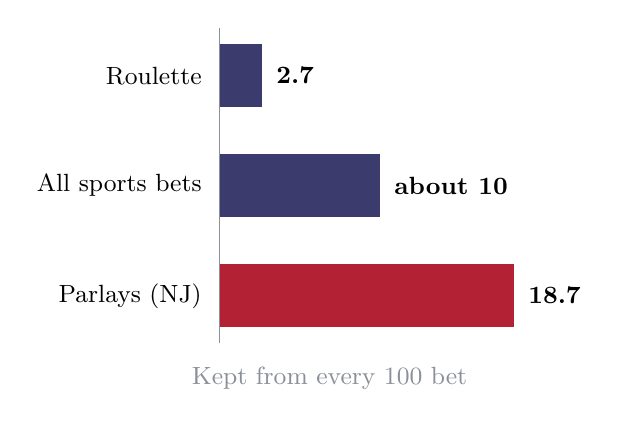
\begin{tikzpicture}[x=0.2cm]
        \foreach \y/\lab/\val/\t/\col in {2.8/Roulette/2.7/2.7/oldblue, 1.4/All sports bets/10.2/about 10/oldblue, 0/Parlays (NJ)/18.7/18.7/oldred} {
          \fill[\col] (0,\y) rectangle (\val,\y+0.8);
          \node[anchor=east, font=\small] at (-0.5,\y+0.4) {\lab};
          \node[anchor=west, font=\small\bfseries] at (\val+0.3,\y+0.4) {\t};
        }
        \draw[muted] (0,-0.2) -- (0,3.8);
        \node[font=\small, text=muted] at (7,-0.65) {Kept from every 100 bet};
      \end{tikzpicture}
    \end{column}
  \end{columns}
  \source{Source: American Gaming Association (2025); InGame (New Jersey, 2025 to date). Roulette: European wheel.}
\end{frame}

\begin{frame}{Who pays?}
  \large In Connecticut, \alert{1.8\%} of people are problem gamblers.\\[0.8em]
  \textbf{What share of sports betting money comes from them?}\\[1.2em]
  \Large A) 5\% \qquad B) 20\% \qquad C) \only<1>{51\%}\only<2->{\ans{51\%}}
  \source{Source: Gemini Research for the State of Connecticut (2024), estimated from what gamblers said they spent.}
\end{frame}

\begin{thinkframe}
  {\color{oldred}\textbf{Think}}\\[0.8em]
  If half your money comes from addicts,\\do you want them to stop?
\end{thinkframe}

% =====================================================================
\section{Addiction}

\begin{frame}{Habit or addiction?}
  \relax{\large\color{muted} Show fingers: 1 = fine, 5 = serious problem\par}
  \vspace{0.8em}
  \begin{itemize}\setlength{\itemsep}{0.8em}\large
    \item<1-> Lotto every week, \texteuro 2
    \item<2-> Bets more to win it back
    \item<3-> Lies about losing
    \item<4-> Plays to forget problems
    \item<5-> Borrows from Grandma to bet
  \end{itemize}
\end{frame}

\begin{frame}{When is it an addiction?}
  \relax{\large\color{muted} Four or more signs in a year\par}
  \vspace{0.8em}
  \begin{itemize}\setlength{\itemsep}{0.8em}\large
    \item Needs bigger and bigger bets
    \item \alert{Can't stop}, restless without it
    \item \alert{Chases losses}
    \item Lies about it
    \item Loses friends, school, job
  \end{itemize}
  \source{Source: DSM-5 (nine criteria, shortened), via Gesundheit \"Osterreich.}
\end{frame}

\begin{frame}{It's a brain thing}
  \begin{itemize}\setlength{\itemsep}{0.9em}\large
    \item Same category as drug addiction
    \item \alert{Dopamine}: excitement \emph{before} the result
    \item Unpredictable rewards hook us
    \item Like scrolling, like loot boxes
    \item Not weakness, not stupidity
  \end{itemize}
  \source{Category: DSM-5, ``substance-related and addictive disorders''.}
\end{frame}

\begin{frame}{Chasing}
  \large US online sports bettors who have ``chased'' a loss:\\[0.7em]
  {\fontsize{36}{42}\selectfont\bfseries\color{oldred}\only<1>{?}\only<2->{60\%}}\\[0.9em]
  \onslide<3->{\begin{itemize}\setlength{\itemsep}{0.6em}
    \item One year earlier: 52\%
    \item Felt bad or ashamed: 43\%
    \item Asked for help: 15\%
  \end{itemize}}
  \source{Source: Siena / St.\ Bonaventure survey (April 2026).}
\end{frame}

\begin{frame}{Higher or lower? Austria}
  \renewcommand{\arraystretch}{1.7}\centering
  \begin{tabular}{@{}lcl@{}}
    Adults and teens 15+ with a problem & \textbf{2\%?} & \onslide<2->{\ans{Higher: 4\%} (about 300,000)} \\
    Men aged 15--34 with a problem & \textbf{5\%?} & \onslide<3->{\ans{Higher: 9.7\%}} \\
    Boys 14--17 who gambled last year & \textbf{20\%?} & \onslide<4->{\ans{Lower: 16\%}} \\
    Girls 14--17 who gambled last year & \textbf{10\%?} & \onslide<5->{\ans{Lower: 4\%}} \\
  \end{tabular}
  \source{Source: Gesundheit \"Osterreich, Epidemiologiebericht Sucht 2025 (self-reported; 2022 population survey and ESPAD 2024 school survey).}
\end{frame}

\begin{frame}{The USA and Austria}
  \renewcommand{\arraystretch}{1.6}
  \begin{tabular}{@{}>{\raggedright\arraybackslash}p{0.27\textwidth}>{\raggedright\arraybackslash}p{0.32\textwidth}>{\raggedright\arraybackslash}p{0.33\textwidth}@{}}
    \toprule
     & \textbf{\color{oldblue}USA} & \textbf{\color{austria}Austria} \\
    \midrule
    Who decides & Each state & Federal + Bundesland \\
    Minimum age & Usually 21 (some 18) & 18 \\
    Sports betting is & Gambling & \leavevmode\alert{Not} legally gambling \\
    Boys who gambled & 36\% (ages 11--17) & 16\% (ages 14--17) \\
    \bottomrule
  \end{tabular}
  \source{Source: Gesundheit \"Osterreich (2025); Common Sense Media (Jan.\ 2026). The boys' figures use different ages and definitions.}
\end{frame}

\begin{frame}{Design the law}
  \relax{\large\color{muted} You are the government. Pick one and defend it.\par}
  \vspace{0.8em}
  \begin{itemize}\setlength{\itemsep}{0.9em}\large
    \item Ban all gambling ads
    \item Maximum \texteuro 100 loss per day
    \item No phone betting
    \item Ban VIP programs
  \end{itemize}
\end{frame}

\begin{frame}{If it stops being fun}
  \begin{itemize}\setlength{\itemsep}{0.9em}\large
    \item Talk to someone you trust
    \item Spielsuchthilfe Wien: \alert{01 544 13 57}
    \item \href{https://genuggespielt.at}{genuggespielt.at} (anonymous, free)
    \item Families can call too
  \end{itemize}
  \source{Source: spielsuchthilfe.at.}
\end{frame}

% =====================================================================
\section{Grammar Casino}

\begin{frame}{Grammar Casino}
  \begin{itemize}\setlength{\itemsep}{0.9em}\large
    \item Groups start with \alert{500 points}
    \item Is the sentence correct?
    \item Bet, then vote
    \item Your points go to blackjack
  \end{itemize}
\end{frame}

\casino{1}{He betted all his money on Rapid.}{He \ans{bet} all his money on Rapid.}
\casino{2}{The money he had won, he spent within a week.}{\cright}
\casino{3}{The odds are against you.}{\cright}
\casino{4}{I have played poker since three years.}{I have played poker \ans{for} three years.}
\casino{5}{The number of teenagers who gamble online have increased.}{The number of teenagers who gamble online \ans{has} increased.}
\casino{6}{If I would win the lottery, I would buy a house.}{If I \ans{won} the lottery, I would buy a house.}
\casino{7}{She has been gambling online for two years.}{\cright}
\casino{8}{He denied to have a gambling problem.}{He denied \ans{having} a gambling problem.}
\casino{9}{Sports betting is very popular in Austria.}{\cright}
\casino{10}{I am agree that sports betting should be banned.}{I \ans{agree} that sports betting should be banned.}
\casino{11}{The house always wins in the long run.}{\cright}
\casino{12}{He promised to stop, but he didn't stopped.}{He promised to stop, but he didn't \ans{stop}.}
\casino{13}{Young men are more likely to bet on sports than women.}{\cright}
\casino{14}{Gambling can become a serious addiction.}{\cright}

% =====================================================================
\section{Final Activity: Blackjack}

\begin{frame}{Blackjack in 30 seconds}
  \begin{columns}[c,onlytextwidth]
    \begin{column}{0.55\textwidth}
      \begin{itemize}\setlength{\itemsep}{0.8em}\large
        \item Closest to \alert{21} wins
        \item Over 21: \alert{bust}
        \item J, Q, K = 10
        \item Ace = 1 or 11
        \item Hit or stand?
      \end{itemize}
    \end{column}
    \begin{column}{0.4\textwidth}
      \centering
      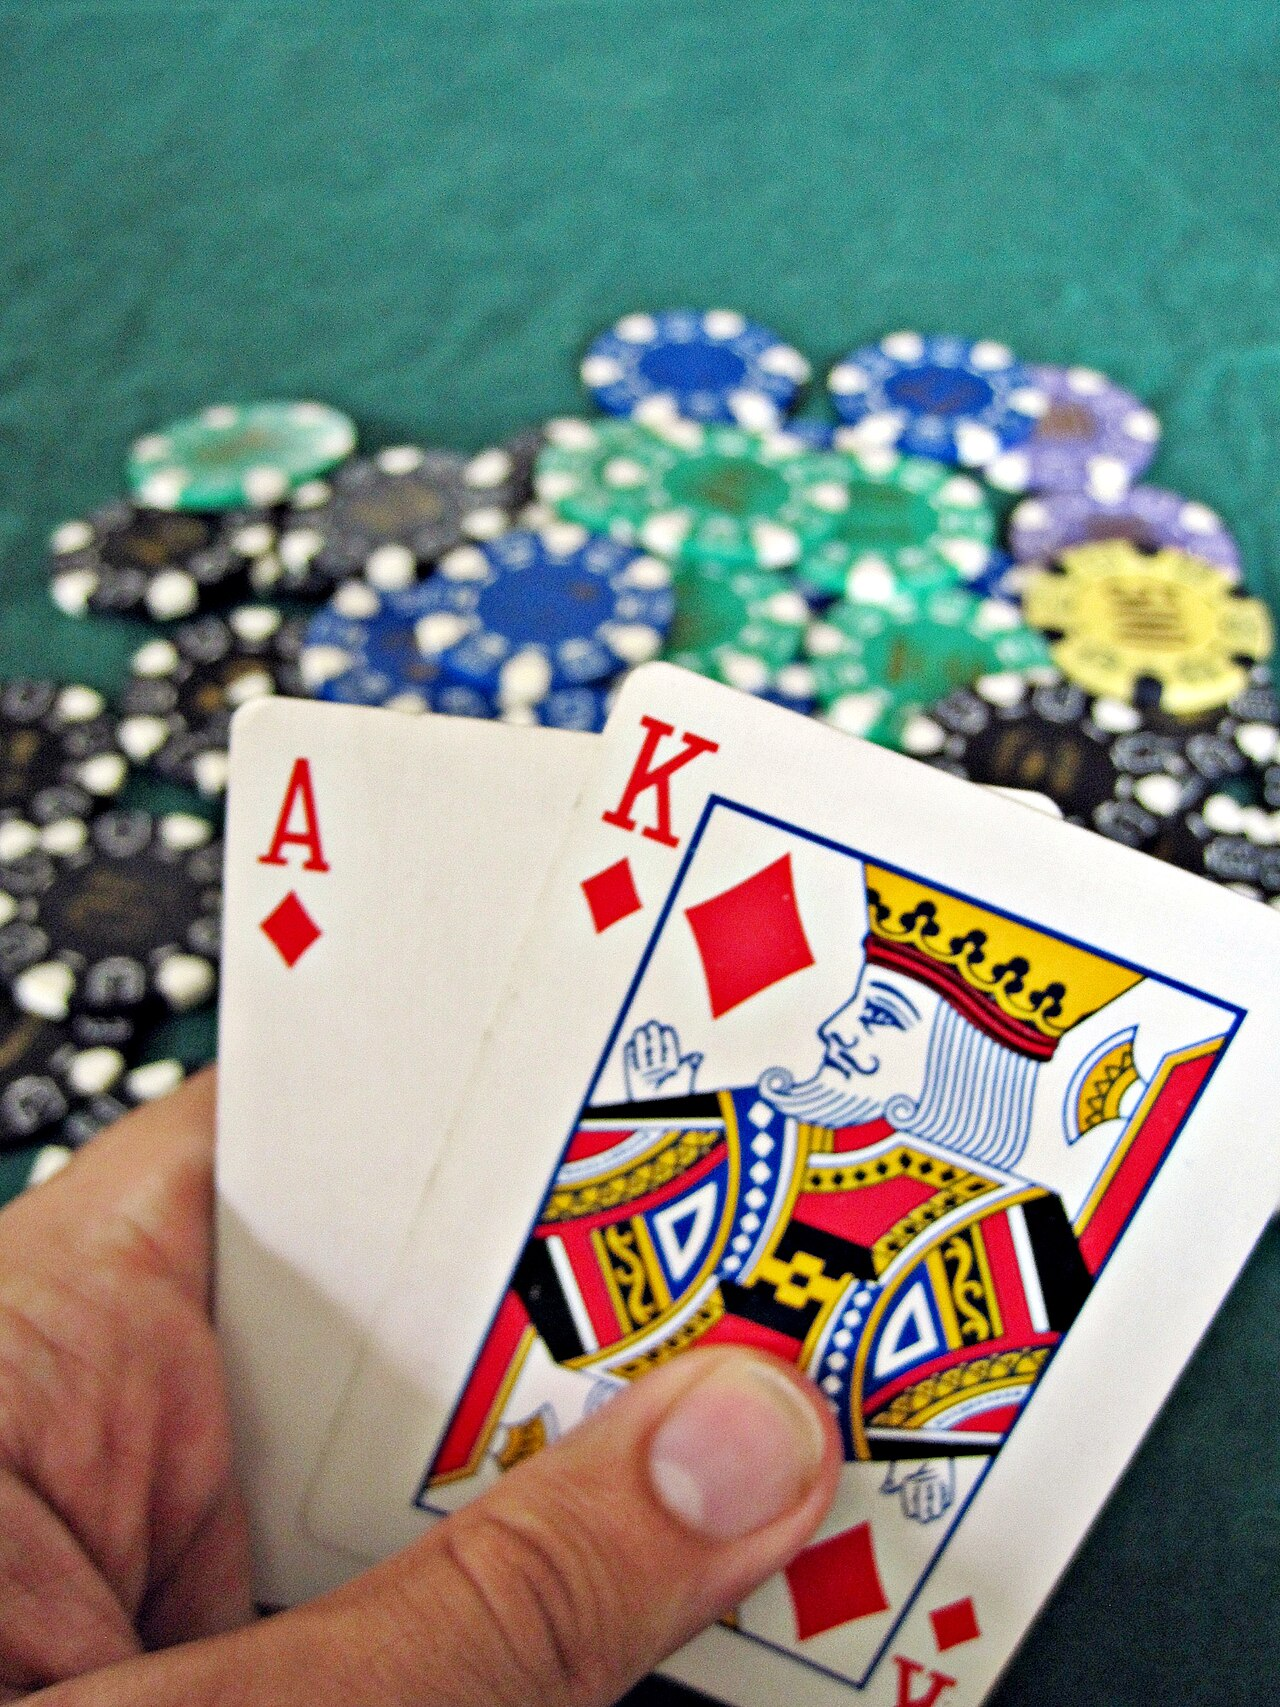
\includegraphics[height=4.9cm]{blackjack.jpg}\\[0.2em]
      {\tiny\color{muted} Photo: Images Money, CC BY 2.0\par}
    \end{column}
  \end{columns}
\end{frame}

\begin{frame}{Let's play}
  \centering
  {\LARGE\bfseries\href{https://noahfried.github.io/slides/blackjack/}{noahfried.github.io/slides/blackjack}}\\[1.4em]
  \begin{minipage}{0.6\textwidth}
  \begin{itemize}\setlength{\itemsep}{0.8em}\large
    \item Four groups, same table
    \item Rounds 1--4: normal blackjack
    \item Round 5: a \alert{special offer}\ldots
  \end{itemize}
  \end{minipage}
\end{frame}

\begin{frame}[plain]
  \vfill
  \centering
  
\begin{tikzpicture}
    \node[fill=oldred, text=white, rounded corners=12pt, inner sep=24pt, align=center]
      {{\fontsize{26}{30}\selectfont\bfseries SPECIAL OFFER!}\\[0.9em]{\Large NEW: side bets}\\[1em]{\fontsize{26}{30}\selectfont\bfseries Win up to 250 to 1!}};
  \end{tikzpicture}\\[1.2em]
  {\Large\color{navy} Want one? Yes or no}
  \vfill
\end{frame}

\begin{frame}{What did we just sell you?}
  \centering
  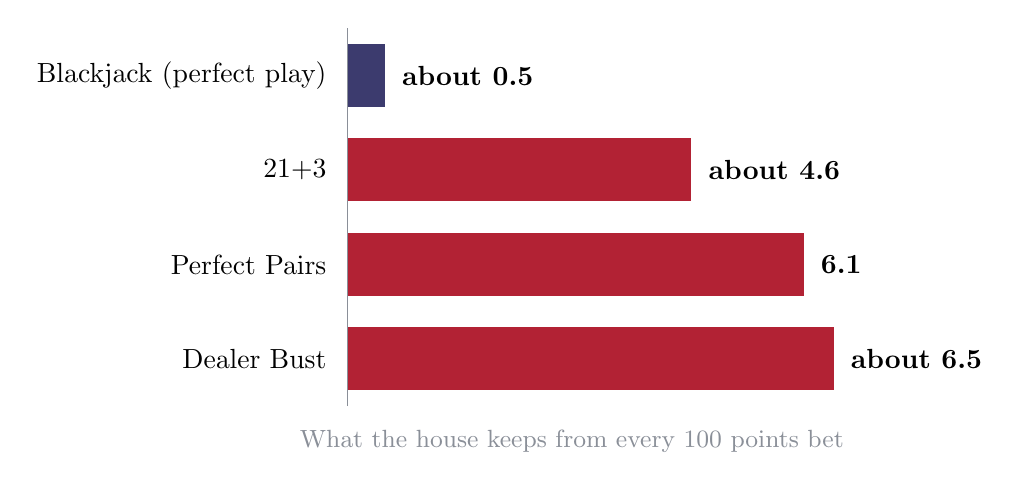
\begin{tikzpicture}[x=0.95cm]
    \foreach \y/\lab/\val/\t/\col in {3.6/{Blackjack (perfect play)}/0.5/about 0.5/oldblue, 2.4/21+3/4.6/about 4.6/oldred, 1.2/Perfect Pairs/6.1/6.1/oldred, 0/Dealer Bust/6.5/about 6.5/oldred} {
      \onslide<2->{\fill[\col] (0,\y) rectangle (\val,\y+0.8);
      \node[anchor=west, font=\bfseries] at (\val+0.1,\y+0.4) {\t};}
      \node[anchor=east] at (-0.15,\y+0.4) {\lab};
    }
    \draw[muted] (0,-0.2) -- (0,4.6);
    \node[text=muted, font=\small] at (3,-0.65) {What the house keeps from every 100 points bet};
  \end{tikzpicture}
  \source{Side bets calculated for this app's rules (six decks).}
\end{frame}

\begin{frame}{Did the house win?}
  \begin{itemize}\setlength{\itemsep}{0.9em}\large
    \item Who has more than before?
    \item Who chased a loss?
    \item Who wanted one more round?
    \item Which trick worked on you?
  \end{itemize}
\end{frame}

\end{document}
